\documentclass[12pt, a4paper, oneside]{Thesis} % Paper size, default font size and one-sided paper
\usepackage{wrapfig}
\usepackage{lscape}
\usepackage{rotating}
\usepackage{graphicx}
\usepackage{caption}
\usepackage{amsmath}

\usepackage{}


\usepackage{lineno,hyperref}
\modulolinenumbers[5]


\usepackage{amssymb}
\usepackage{graphicx}
\usepackage{array}
\usepackage{float}
\usepackage{placeins}
\usepackage{stackengine}
\usepackage{url}
\usepackage{numprint}
\usepackage{caption}

\usepackage{booktabs}  
\usepackage{siunitx}
%\usepackage[showframe=false]{geometry}
\usepackage{subfigure}

\nprounddigits{3}
\newcolumntype{P}[1]{>{\centering\arraybackslash}p{#1}}
\newcolumntype{M}[1]{>{\centering\arraybackslash}m{#1}}

\setstackEOL{\#}
\setstackgap{L}{12pt}


%\usepackage{subcaption} %incompatible with subfig
\graphicspath{{Pictures/}} % Specifies the directory where pictures are stored
\usepackage{natbib} % Use the natbib reference package - read up on this to edit the reference style; if you want text (e.g. Smith et al., 2012) for the in-text references (instead of numbers), remove 'numbers' v

\hypersetup{urlcolor=black, colorlinks=false} % Colors hyperlinks in blue - change to black if annoyingv`	

\thesistitle{POS Blockchain with Dynamically Changing Validators}
\supervisor{Prof. Sandip Chakraborty and Dr. Pralhad Deshpande}
\degree{Bachelor of Technology}
\degreemajor{Computer Science and Engineering}
\authors{Nishant Baranwal Somy}
\rollno{15CS30044}
\university{Indian Institute of Technology Kharagpur}
\department{Department of Computer Science and Engineering}
\unisite{http://www.iitkgp.ac.in}
\depsite{http://www.cse.iitkgp.ac.in}
\placeshrt{Kharagpur}
\placelng{Kharagpur - 721302, India}
\datesub{November 12, 2018}
\datesig{November 12, 2018}
\semsub{Autumn Semester, 2018-19}
%\keywords{Steel Structure}
\coursecd{Project-I (CS47007) }

\title{\ttitle} % Defines the thesis title - don't touch this
\begin{document}
%\makeatletter
%\renewcommand*{\NAT@nmfmt}[1]{\textsc{#1}}
%\makeatother

% prints author names as small caps


\frontmatter % Use roman page numbering style (i, ii, iii, iv...) for the pre-content pages

\setstretch{1.6} % Line spacing of 1.6 (double line spacing)

% Define the page headers using the FancyHdr package and set up for one-sided printing
\fancyhead{} % Clears all page headers and footers
\rhead{\thepage} % Sets the right side header to show the page number
\lhead{} % Clears the left side page header

%\pagestyle{fancy} % Finally, use the "fancy" page style to implement the FancyHdr headers

\newcommand{\HRule}{\rule{\linewidth}{0.5mm}} % New command to make the lines in the title page

% PDF meta-data
\hypersetup{pdftitle={\ttitle}}
\hypersetup{pdfsubject=\subjectname}
\hypersetup{pdfauthor=\authornames}
\hypersetup{pdfkeywords=\keywordnames}

%----------------------------------------------------------------------------------------
%	TITLE PAGE
%----------------------------------------------------------------------------------------
\maketitle
%\titlepg % Add a gap in the Contents, for aesthetics

\clearpage % Start a new page

%----------------------------------------------------------------------------------------
%	DECLARATION PAGE
%	Your institution may give you a different text to place here
%----------------------------------------------------------------------------------------


\Declaration% Add a gap in the Contents, for aesthetics


%----------------------------------------------------------------------------------------
%	CERTIFICATE PAGE
%----------------------------------------------------------------------------------------

\addtotoc{Certificate} % Add the "Abstract" page entry to the Contents

\certificate{\addtocontents{toc}{} % Add a gap in the Contents, for aesthetics

}

\clearpage % Start a new page

%----------------------------------------------------------------------------------------
%	ABSTRACT PAGE
%----------------------------------------------------------------------------------------

%\addtotoc{Abstract} % Add the "Abstract" page entry to the Contents

%\abstract{\addtocontents{toc}{} % Add a gap in the Contents, for aesthetics

%Enter content here. 
%}

%\clearpage % Start a new page



%----------------------------------------------------------------------------------------
%	ACKNOWLEDGEMENTS
%----------------------------------------------------------------------------------------

%\setstretch{1.3} % Reset the line-spacing to 1.3 for body text (if it has changed)

%\acknowledgements{\addtocontents{toc}{}%\vspace{1em}} % Add a gap in the Contents, for aesthetics

%Enter acknowledgement content here.

%}
%\clearpage % Start a new page

%----------------------------------------------------------------------------------------
%	LIST OF CONTENTS/FIGURES/TABLES PAGES
%----------------------------------------------------------------------------------------

\pagestyle{fancy} % The page style headers have been "empty" all this time, now use the "fancy" headers as defined before to bring them back

\lhead{\emph{Contents}} % Set the left side page header to "Contents"
\tableofcontents % Write out the Table of Contents

%\lhead{\emph{List of Figures}} % Set the left side page header to "List of Figures"
%\listoffigures % Write out the List of Figures

%\lhead{\emph{List of Tables}} % Set the left side page header to "List of Tables"
%\listoftables % Write out the List of Tables

%----------------------------------------------------------------------------------------
%	ABBREVIATIONS
%----------------------------------------------------------------------------------------

% \clearpage % Start a new page

% \setstretch{1.5} % Set the line spacing to 1.5, this makes the following tables easier to read

% \lhead{\emph{Abbreviations}} % Set the left side page header to "Abbreviations"
% \listofsymbols{ll} % Include a list of Abbreviations (a table of two columns)
% {
% \textbf{FEA} & \textbf{F}inite \textbf{E}lement \textbf{A}nalysis \\
% \textbf{FEM} & \textbf{F}inite \textbf{E}lement \textbf{M}ethod \\
% \textbf{LVDT} & \textbf{L}inear \textbf{V}ariable \textbf{D}ifferential \textbf{T}ransformer \\
% \textbf{RC} & \textbf{R}einforced \textbf{C}oncrete
% %\textbf{Acronym} & \textbf{W}hat (it) \textbf{S}tands \textbf{F}or \\
% }

%----------------------------------------------------------------------------------------
%	PHYSICAL CONSTANTS/OTHER DEFINITIONS
%----------------------------------------------------------------------------------------
%
%\clearpage % Start a new page
%
%\lhead{\emph{Physical Constants}} % Set the left side page header to "Physical Constants"
%
%\listofconstants{lrcl} % Include a list of Physical Constants (a four column table)
%{
%Speed of Light & $c$ & $=$ & $2.997\ 924\ 58\times10^{8}\ \mbox{ms}^{-\mbox{s}}$ (exact)\\
%% Constant Name & Symbol & = & Constant Value (with units) \\
%}

%----------------------------------------------------------------------------------------
%	SYMBOLS
%----------------------------------------------------------------------------------------

% \clearpage % Start a new page

% \lhead{\emph{Symbols}} % Set the left side page header to "Symbols"

% \listofnomenclature{lll} % Include a list of Symbols (a two column table)
% {
% $D^{el}$ & elasticity tensor \\
% $\sigma$ & stress tensor \\
% $ \varepsilon $ & strain tensor \\
% % Symbol & Name & Unit \\

% }

%----------------------------------------------------------------------------------------
%	DEDICATION
%----------------------------------------------------------------------------------------
%
%\setstretch{1.3} % Return the line spacing back to 1.3
%
%\pagestyle{empty} % Page style needs to be empty for this page
%
%\dedicatory{For/Dedicated to/To my\ldots} % Dedication text
%
%\addtocontents{toc}{\vspace{2em}} % Add a gap in the Contents, for aesthetics

%----------------------------------------------------------------------------------------
%	THESIS CONTENT - CHAPTERS
%----------------------------------------------------------------------------------------

\mainmatter % Begin numeric (1,2,3...) page numbering

\pagestyle{fancy} % Return the page headers back to the "fancy" style

% Include the chapters of the thesis as separate files from the Chapters folder
% Uncomment the lines as you write the chapters

% Introduction - A bit description of Blockchain and the problem statement you are working on
% Chapter Template

\chapter{Introduction} % Main chapter title

\label{Chapter 1} % Change X to a consecutive number; for referencing this chapter elsewhere, use \ref{ChapterX}

\lhead{Chapter 1. \emph{Introduction}} % Change X to a consecutive number; this is for the header on each page - perhaps a shortened title

%----------------------------------------------------------------------------------------
%	SECTION 1
%----------------------------------------------------------------------------------------
\section{What is a blockchain?}



A blockchain is a growing list of records, called blocks, which are linked using cryptography. Each block contains a cryptographic hash of the previous block, a timestamp, and transaction data (generally represented as a merkle tree root hash).

By design, a blockchain is resistant to modification of the data. It is "an open, distributed ledger that can record transactions between two parties efficiently and in a verifiable and permanent way". For use as a distributed ledger, a blockchain is typically managed by a peer-to-peer network collectively adhering to a protocol for inter-node communication and validating new blocks. Once recorded, the data in any given block cannot be altered retroactively without alteration of all subsequent blocks, which requires consensus of the network majority. Although blockchain records are not unalterable, blockchains may be considered secure by design and exemplify a distributed computing system with high Byzantine fault tolerance. Decentralized consensus has therefore been claimed with a blockchain.

\section{Problem Statement}

A blockchain system's throughput depends on the number of nodes participating in the validation of a transaction. More the number of nodes means more resistance to faults but resulting in higher latency and lower throughputs. The objective of this project is to propose a blockchain system where the number of validators is determined by the market dynamics.


% \paragraph{Literature Survey}

% This is a sample. Write about referred papers. Cite like this \citep{nip2010cyclic}. Another example would be this \citep{nip2010extremely}. More citations like this \citep{bird2004evaluating}, \citep {tremblay2003seismic} and \citep {alhamaydeh2016key}.

% \paragraph{Research gaps}
% Typically include research gaps for your study. 
% \paragraph{Objective}
% Similarly objectives of study. 
% \paragraph{Scope}
% Define scope of study. 
% \paragraph{An algorithm}
% How you could refer to figures: This is an example. (Refer \ref{fig5}). You can add equations like this Eq. (\ref{eq1})
% \begin{equation}
% \label{eq1}
%   SDR = sd(T) - \sum_{i}\frac{{T}_{i}}{|T|}\times sd({T}_{i})
% \end{equation}

% \begin{figure}[]
% \centering
% 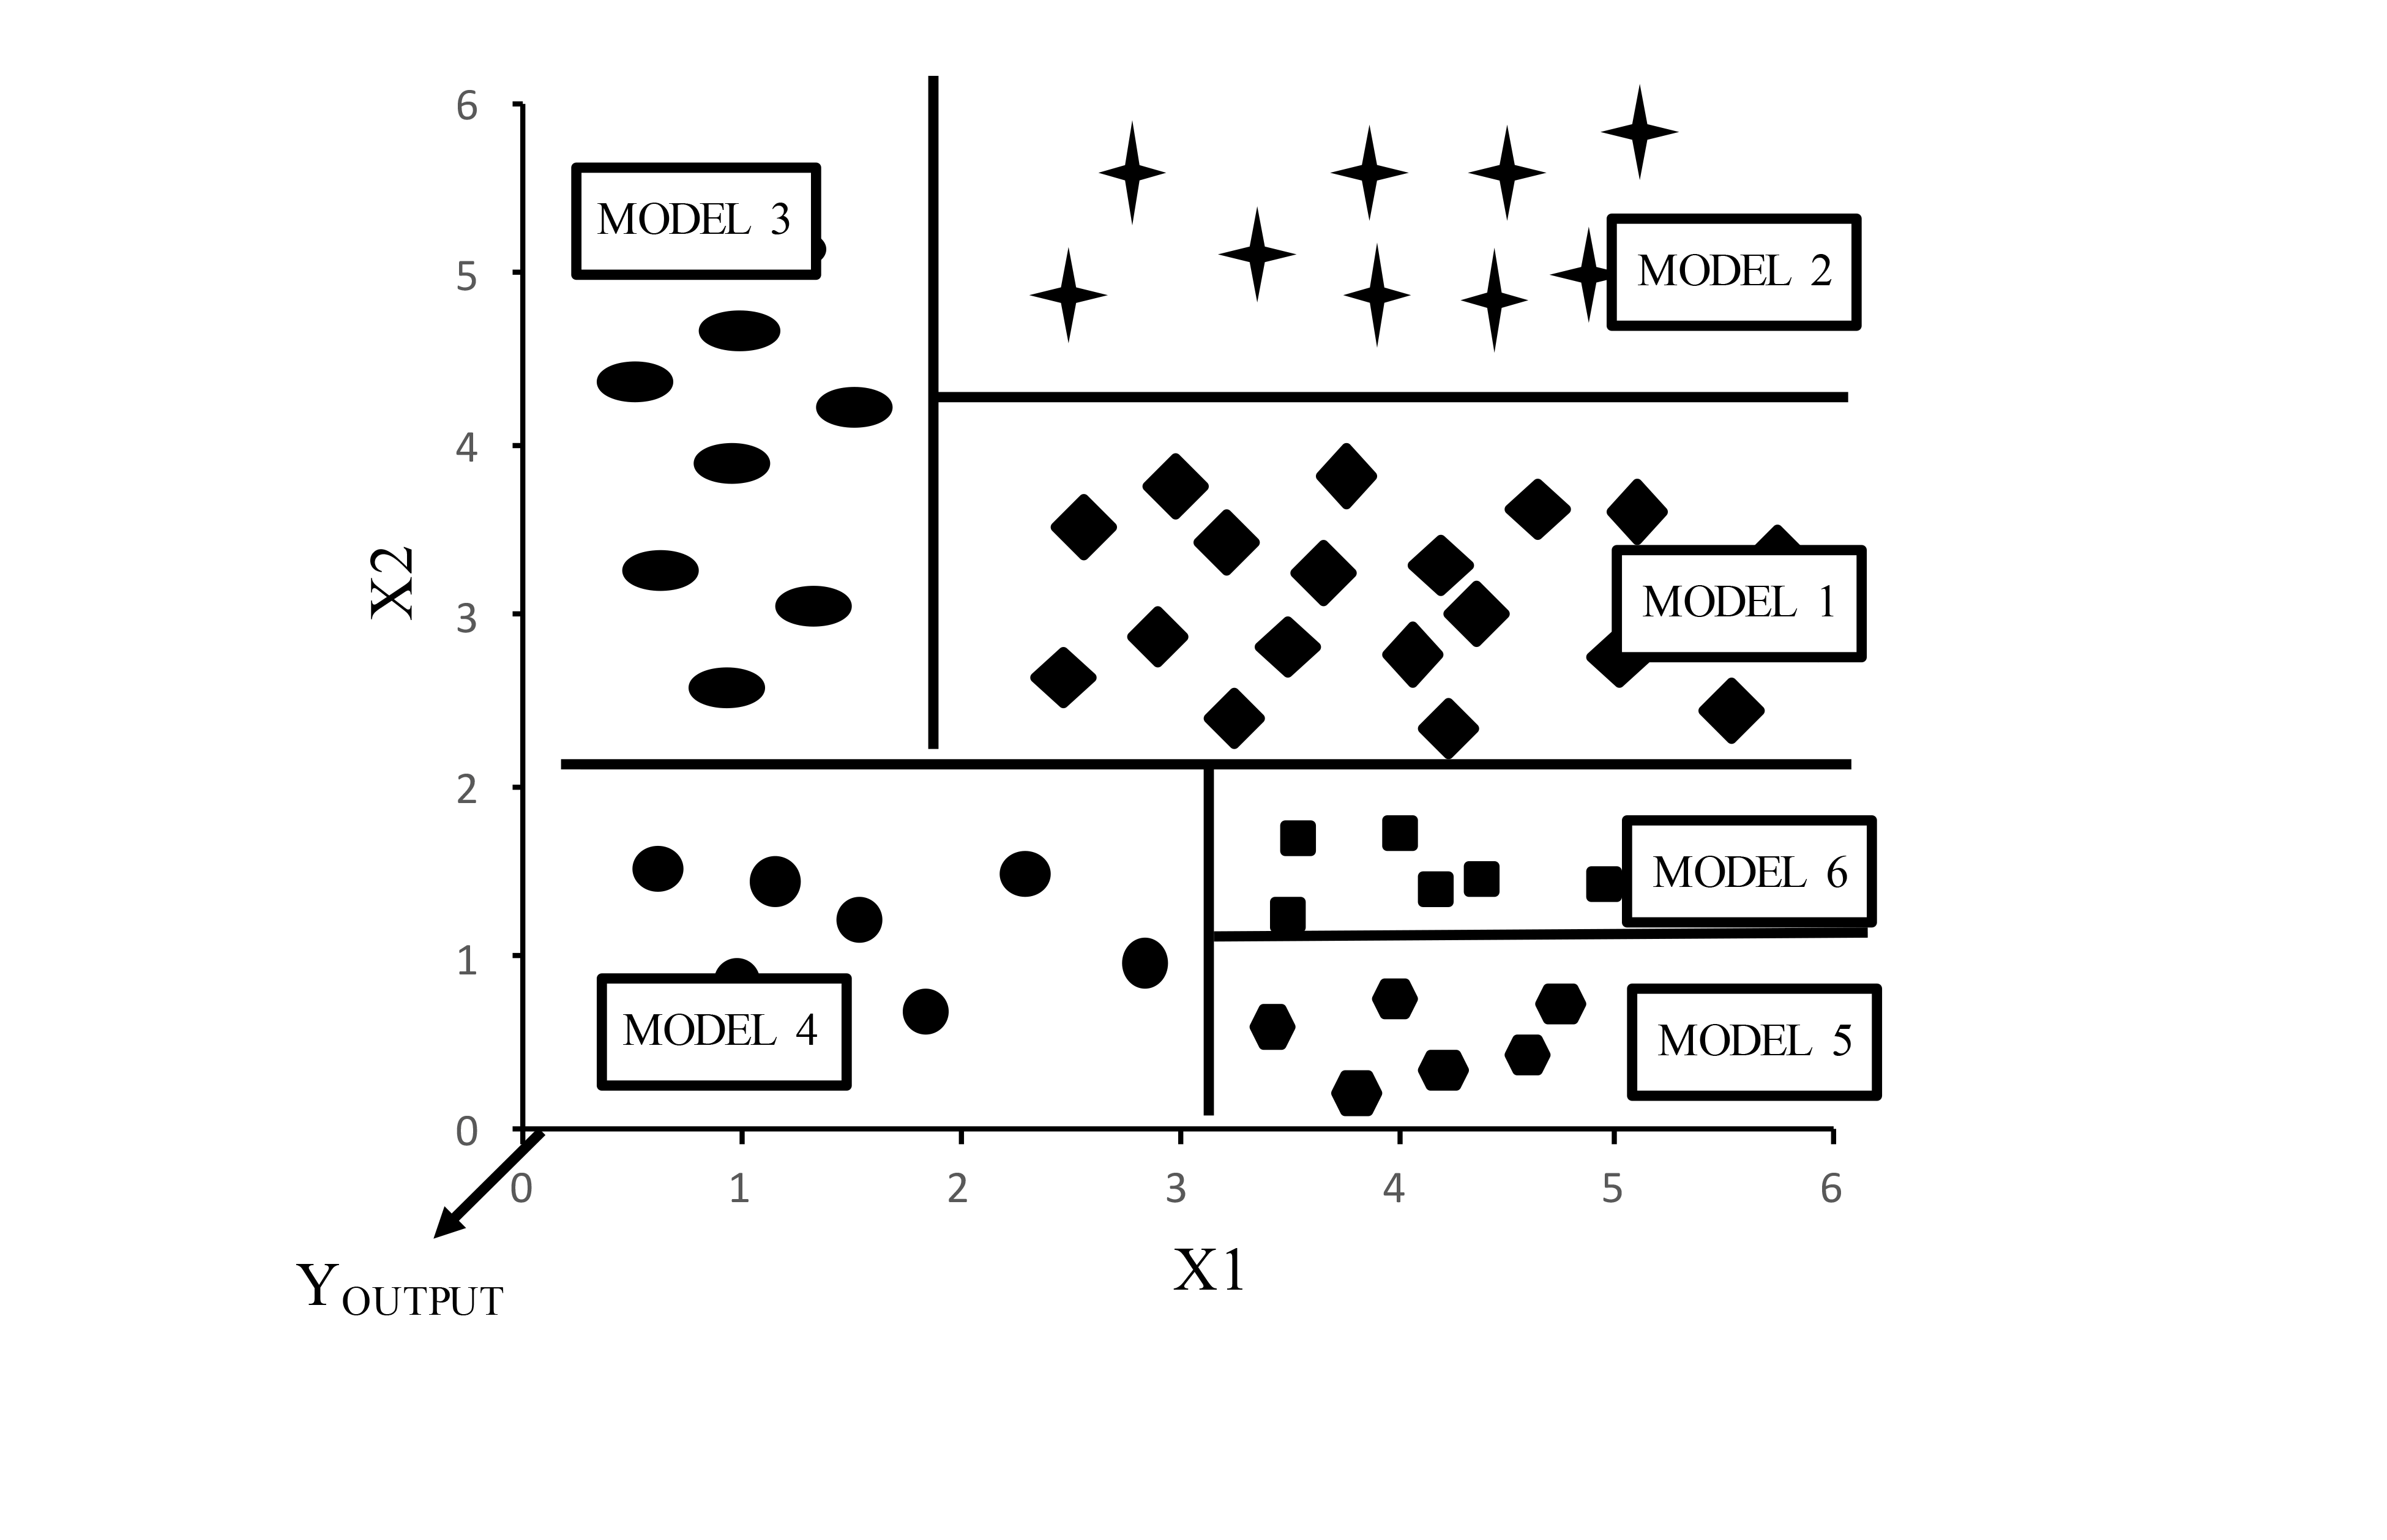
\includegraphics[height=7cm]{splits.png}
% \caption{Splitting of the input space (X1 x X2) by M5' model tree algorithm}
% \label{fig5}
% \end{figure}

% \section{Adding another section}
% You can show a lot of figures together like these Figures \ref{fig61}, \ref{fig62}, \ref{fig63} below.
% \begin{figure} [!htbp]
% \centering    
% \subfigure[Caption1]{\label{fig61}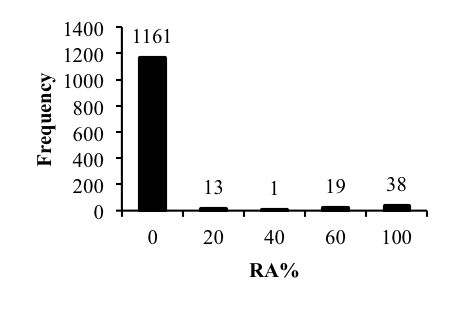
\includegraphics[width=42mm]{data1.png}}
% \subfigure[Caption2]{\label{fig62}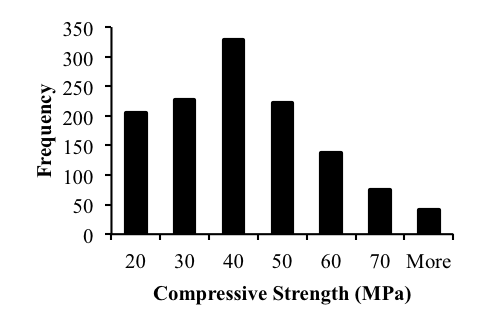
\includegraphics[width=42mm]{data2.png}}
% \subfigure[Caption3]{\label{fig63}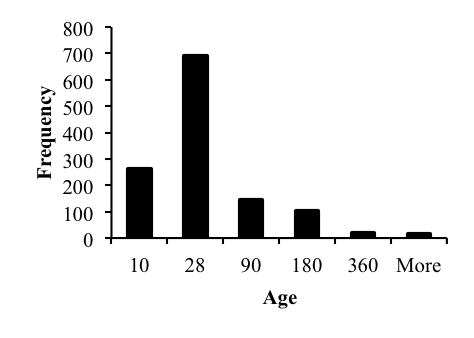
\includegraphics[width=42mm]{data3.png}}
% \caption{Figures sample}
% \end{figure}
% You can add lists into the text like this. 
% \begin{itemize}
% \settowidth{\leftmargin}{{\Large$\square$}}\advance\leftmargin\labelsep
% \itemsep3pt\relax
% \renewcommand\labelitemi{{\lower1pt\hbox{\small$\square$}}}
% \item	Some sample text item 1. 
% \item You may refer to tables \ref{tab1} 
% \item Or figures \ref{fig61}
% \end{itemize}

% Tables can be added like this
% \begin{table}[!htbp]
% \centering
% \caption{Sample table}
% \label{tab1}
% \begin{tabular}{llll}

% \hline
% Column 1 & Column 2 & Column 3       \\\hline
% 1         & Data1 & 13.41179 & 0.9492839 \\
% 2            & Data2 & 13.39824 & 0.9492952\\\hline
% \end{tabular}
% \end{table}



%% Discussion - Discuss the issues that you have got in the system, an idea about how you are trying to solve those. 
% Chapter Template

\chapter{Discussion} % Main chapter title

\label{Chapter 4} % Change X to a consecutive number; for referencing this chapter elsewhere, use \ref{ChapterX}

\lhead{Chapter 4. \emph{Discussion}} % Change X to a consecutive number; this is for the header on each page - perhaps a shortened title

\section{Problems in System Design}

Here, we note some of the problems and boundary cases that might occur during the design and execution of the system and we try to give some plausible solutions.

\begin{enumerate}
    \item We know that CashCoins are liquid and can be transferred from one user to another. But, what if a user wants to transfer his voting rights to another user? If this user simply transfers it then he would also have to share the public-private key associated with this coin, but these are digital quantities and can be copied and can lead to the free-rider problem.\\
    Solution : Here, we assume that BondCoins are illiquid and non-transferable. If some user wants to transfer them, then he first has to convert the Coin to CashCoin and send these to the target user who then can convert these back to a BondCoin. This also avoids the free rider problem as when the target user gets his BondCoin, he would also get a new key pair associated with it.
    \item The bond coins are going to be minted using PoW. Once, all the bond coins are minted, the system adopts PoS system. PoW means we are finding some nonce which satisfies some properties, (In case of bitcoin, it had to be less than a given number). But, here the each bond coin is associated with a public and a private key pair which satisfy their own properties. How does the two gets associated?\\
    Solution : Here, the nonce and key-pairs are not related. A user can get a key pair even when PoS has taken over. We use El Gamal Cryptosystem for getting the private-public key pair associated with the BondCoin. This Cryptosystem is based on Elliptic Curve Cryptography (ECDLP) and provides better security with lesser key size. The Base point is common for all users. The private key can be decided by the winner of the current round randomly and based on it a public key can be chosen. But, once its decided, the user cannot change it and has to wait till the BondCoin matures. If he wants to change it then he would have to convert it to CashCoin and then again to BondCoin to choose a new one.
    \item What happens if a user who already owns a BondCoin wins another round while PoW consensus is active?\\
    Solution : If a user wins another round while PoW consensus is active, then he gets to commit that block but the BondCoin that is minted gets added to his account as CashCoin without any penalty. This is done to make sure that each validators has equal voting rights and hence own only one BondCoin with them.
    \item Here we note that PoW algorithm is only for minting bond coins. So, do the users don’t transact till all the bond coins are minted or does the peer minting the next bond coin becomes the leader for that round and commits the block of transactions to the ledger and once all the minting is over, PoS takes over and only those peers can take part in validation who are holding the bond coins?\\
    Solution : Here, we go with the choice that when the PoW consensus is active, the users can still transact and transaction fees are not taken from them. This is done to invite new users to the system and to increase the validators in the system. To incentivise users to participate in the consensus, the BondCoin minted in the current round is paid to the winner of the current round. Note that even after winning once, the users would still want to participate in the consensus to increase the CashCoins in their account.
    \item Each BondCoin comes with a maturity duration d. How is this maturity duration decided? What happens to the keys of the BondCoin once it gets expired and gets converted into CashCoin?\\
    Solution : Currently, this maturity duration is kept as a constant. Eg: 1 month. And, we plan to decide this value emphirically. Each BondCoin comes with a manufacture date, which is stored in the ledger. Once a BondCoin is expired, it gets added as CashCoins to the user account and the keys become useless. This process takes place the first time user transacts after his BondCoin is expired. If he tries to vote using the old keys then his vote is discarded during the expiration check phase.
    \item Since, the CashCoins are not converted automatically to BondCoins, what happens when there is no BondCoin left in the system?\\
    The situation where no BondCoins are left in the system is hard to occur. As the BondCoins in the system decrease, the transaction fees would decrease. In this case, automatically the demand for BondCoins would increase as the few users who are owners of the last few BondCoin would enjoy more shares of the transaction fees by themselves. But, no BondCoin situation can occur only when the last of BondCoins also got matured automatically and no other user converted their CashCoin into a BondCoin before their expiration which would bring the system to a standstill. If there are no BondCoin in the system then there would be no validators in the system and no user would be able to transact and hence the CashCoins in their account would become useless. In this unlikely situation, we suggest that the PoW system is restarted so that the BondCoins in the system can be increased and users can enjoy transactions without paying the fees and do not have to leave the system.
    \item Why is there a penalty for converting BondCoin to CashCoin? How is its amount fixed?\\
    Solution : The BondCoin is like a contract given to user to participate in the validation process during its maturity period. Its like a fixed deposit done in bank, on which you get the interest during the period but you can use the money only after it matures, if you take the money out before it matures then you have to pay a penalty. In a similar way, this penalty is imposed on those users who want to do away with their responsibility of participating in the validation process. The amount is fixed based on the number of BondCoins currently in the system. More the number of BondCoins, more the penalty.

\end{enumerate}

\section{Plausible attacks}

Here, we assume that the block has been prepared and validators are decided, we only need to consider attacks that can be made while committing this block to the ledger.

\begin{enumerate}
    \item Adversary can be the owner of majority of bond coins. Adversary can make multiple accounts with only enough cash coin to convert them into bond coins.
    \item If in response to above, the bond coins are made larger in number then network attacks would be easier. Adversary may be able to slow down the network or partition some nodes.
    \item Instead of buying the bond coins itself, adversary may hack prominent accounts holding bond coins. It's useful as they are gonna be valid for duration d.
\end{enumerate} 
%% Conçlusion and Future Works. 
% Chapter Template

\chapter{Conclusion and Future Works} % Main chapter title

\label{Chapter 5} % Change X to a consecutive number; for referencing this chapter elsewhere, use \ref{ChapterX}

\lhead{Chapter 5. \emph{Conclusion and Future Works}} % Change X to a consecutive number; this is for the header on each page - perhaps a shortened title

In this report, we saw how the number of validators for a POS system can be dynamic and may be determined by the market parameters. The POS systems were better than POW systems because they don't waste computational power in redundant tasks but POS systems itself has some drawbacks. The proposed system tries to solve some of these drawbacks. The crux of the proposed system lies in the fact that all the validators are given equal voting rights so that adversary is also ripped off of the probabilistic advantage of gaining the control of the system which is prevalent in the recently proposed systems such as Algorand. In this system, gaining half the currency of the system is not enough for the adversary. He must have control over more than half of the BondCoins i.e. more than half of the computation power. And, as these BondCoins come with an expiry, the task of the adversary becomes more difficult.

In future we would like to achieve the following objectives :
\begin{enumerate}
    \item We would like to explore how the system is affected if the maturity duration of a BondCoin is variable
    \item We would like to devise a method to ensure that a minimum number of validators are always there in the network at a given point of time
    \item We would like to explore how the system is affected if the BondCoin is also quantized. For eg : a group of users can combine their CashCoins to get one BondCoin. What would be the final vote of such a group of users?
    \item Till now, we have assumed that all the validators remain active all the time. We would like to explore what happens if some of the validators crash or go offline.
    \item We would like to tackle the geographical scalability of POS protocols and devise a solution for it.
    \item We would like to implement a prototype of the above proposed system and run benchmark tests on it.
    \item We would like to explore how charging fees for conversion of CashCoin to BondCoin affects the economy of the system.
\end{enumerate}
 
%\input{Chapters/Chapter6} 
%\input{Chapters/Chapter7} 

%----------------------------------------------------------------------------------------
%	THESIS CONTENT - APPENDICES
%----------------------------------------------------------------------------------------

\addtocontents{toc}{\vspace{2em}} % Add a gap in the Contents, for aesthetics

% Motivation - Description of PoS based system that motivates the design of a new solution. Specify the requirements on why PoS is not suitable in its current form and give motivation behind the solution architecture. 
% Chapter Template

\chapter{Motivation} % Main chapter title

\label{Chapter 2} % Change X to a consecutive number; for referencing this chapter elsewhere, use \ref{ChapterX}

\lhead{Chapter 2. \emph{Motivation}} % Change X to a consecutive number; this is for the header on each page - perhaps a shortened title

%----------------------------------------------------------------------------------------
%	SECTION 1
%---------------------------------------------------------------------------------------
\section{State Machine Replication}

In computer science, state machine replication or state machine approach is a general method for implementing a fault-tolerant service by replicating servers and coordinating client interactions with server replicas.


Blockchain systems are an example of such a system where a ledger of committed transactions acts as a common state between the replicas. These replicas are also known as miners. In a blockchain system, a leader is chosen to commit the new block to the ledger, and the commit is successful only when a consensus is reached on it. This consensus can be reached via two methods, Proof of Work based consensus or Proof of Stake based consensus.

% \section{Types of faults}

% \subsection{Crash Faults}

% A replica is said to be crash-faulty if it stops all computation and communication.

% \subsection{Byzantine Faults}

% A replica is said to be Byzantine or non-crash faulty if it acts arbitrarily, but cannot break cryptographic primitives we use (crypto- graphic hashes, MACs, message digests and digital signatures).

% \subsection{Network Faults}

% A network fault is defined as the inability of some correct replicas to communicate with each other in a timely manner, that is, when a message exchanged between two correct replicas cannot be delivered and processed within delay $\Delta$, known to all replicas.

\section{Proof Of Work based consensus}

In Proof of Work based consensus, the miners compete against each other to complete transactions on the network and get rewarded. The miners are required to solve a hard problem (Eg : Finding a number which when concatenated with the current block of transactions produces a hash which is less than a given number). Whichever miner solves the problem first becomes the leader for the current round and the number acts as his proof of work. The miner then gets to commit the next block to the ledger. To take over the system, an adversary needs to own more than half of the computation power in the network. This consensus system though secured has certain drawbacks. 
\begin{enumerate}
  \item To make sure that all the miners are updated with the current ledger and to generate the consensus for the next block, it is important for the system to have a minimum amount of delay between commitment of two consecutive blocks. And, as the number of miners grow, this delay increases and hence the latency increases too.
  \item As the number of miners increase in the network, the computation power of the network increases. And hence, the problem has to made harder and harder to solve to match with the delay required to for all miners to be in sync.
  \item As all the miners are trying to solve the same problem and only one comes on top as the winner. A lot of computational power is wasted in doing redundant work.
  \item Miners are also given transaction fees to incentivise them to compete against each other and use the computation power. And, this fees varies over time as the number of validators increase and value of the currency increases.
  \item The blockchain can only support finite number of transactions because as the number of nodes increase, you can only make the problem finitely much harder.
\end{enumerate}

Due to these drawbacks, the blockchain systems today are now adopting Proof of stake consensus protocols.

\section{Proof Of Stake based Consensus}

In a proof of stake system, the creator of the next block is determined by a randomized system that is, in part, dictated by how much of that cryptocurrency a user is holding or, in some cases, how long they have been holding that particular currency. Instead of computational power, as is the case in proof of work, the probability of creating a block and receiving the associated rewards is proportional to a user’s holding of the underlining token or cryptocurrency on the network. Eg : If a set of potential validators was made up of Adam, who is holding 40 tokens, Fil with 30, Tomek with 20 and Daniel with 10, there will be a 40\% chance of Adam being chosen to validate the block and Daniel 10\%, with Tomek and Fil on 20\% and 30\% respectively.

The randomization in a proof of stake system prevents centralization, otherwise the richest individual in the system would always be creating the next block and consistently increasing their wealth and as a result their control of the system. The main advantage of proof of stake, over a system such as proof of work, is that it uses considerably less energy and as a result is more cost effective. It is well documented that each Bitcoin transaction, which uses a proof of work system, can require as much electricity as an average Dutch household does in two weeks. This is both ineffective and unsustainable.

So, in total Proof of Stake consensus has following major benefits over Proof of Work consensus :

\begin{enumerate}
    \item It requires far less electricity to work as miners now don't need to waste computation power in doing redundant work of solving a hard problem.
    \item As the proof of stake system is so much more cost effective there is less of a need to release too many new coins as a means of incentivizing miners to maintain the network. This helps to keep the price of a particular coin more stable.
    \item The number of transactions that can be supported now is not finite, as now the miners don't have to solve a hard problem for proof of work
    \item Every node doesn't need to participate now in the validation. Only specially designated nodes participate in the consensus protocol.
    \item As the requirement of proof of work is removed, and the system is validated by a finite set of nodes, the system can work faster giving rise to higher throughputs and lower latencies. 
\end{enumerate}

\section{Drawbacks of POS consensus}

Even though the POS consensus has so many benefits, it has some of its drawbacks too. Following are some of them :

\begin{enumerate}
    \item The conventional POS systems are not as open as POW systems, one needs permission of the present member of the system to become part of the system or leave the system altogether
    \item The performance and trustworthiness of the system is largely affected by the number of validators present in the system. As the number of validators increase, trustworthiness of the system increases but the performance of the system goes down. POW systems have lower latencies but they maintain an average. Another reason why POS systems are designed to be closed.
    \item POS systems have geographical scalability issues. As the hops between the nodes increase, the performance of the system goes down. This happens because POS systems try to perform as better as possible but as the distance increases, it takes more time to form the consensus.
\end{enumerate}
Through this project, we are trying to tackle the first two issues of the Proof of Stake blockchain systems. In simple terms, our objective is to determine what's the correct number of validators in the system using market dynamics.

% \paragraph{Literature Survey}

% This is a sample. Write about referred papers. Cite like this \citep{nip2010cyclic}. Another example would be this \citep{nip2010extremely}. More citations like this \citep{bird2004evaluating}, \citep {tremblay2003seismic} and \citep {alhamaydeh2016key}.

% \paragraph{Research gaps}
% Typically include research gaps for your study. 
% \paragraph{Objective}
% Similarly objectives of study. 
% \paragraph{Scope}
% Define scope of study. 
% \paragraph{An algorithm}
% How you could refer to figures: This is an example. (Refer \ref{fig5}). You can add equations like this Eq. (\ref{eq1})
% \begin{equation}
% \label{eq1}
%   SDR = sd(T) - \sum_{i}\frac{{T}_{i}}{|T|}\times sd({T}_{i})
% \end{equation}

% \begin{figure}[]
% \centering
% 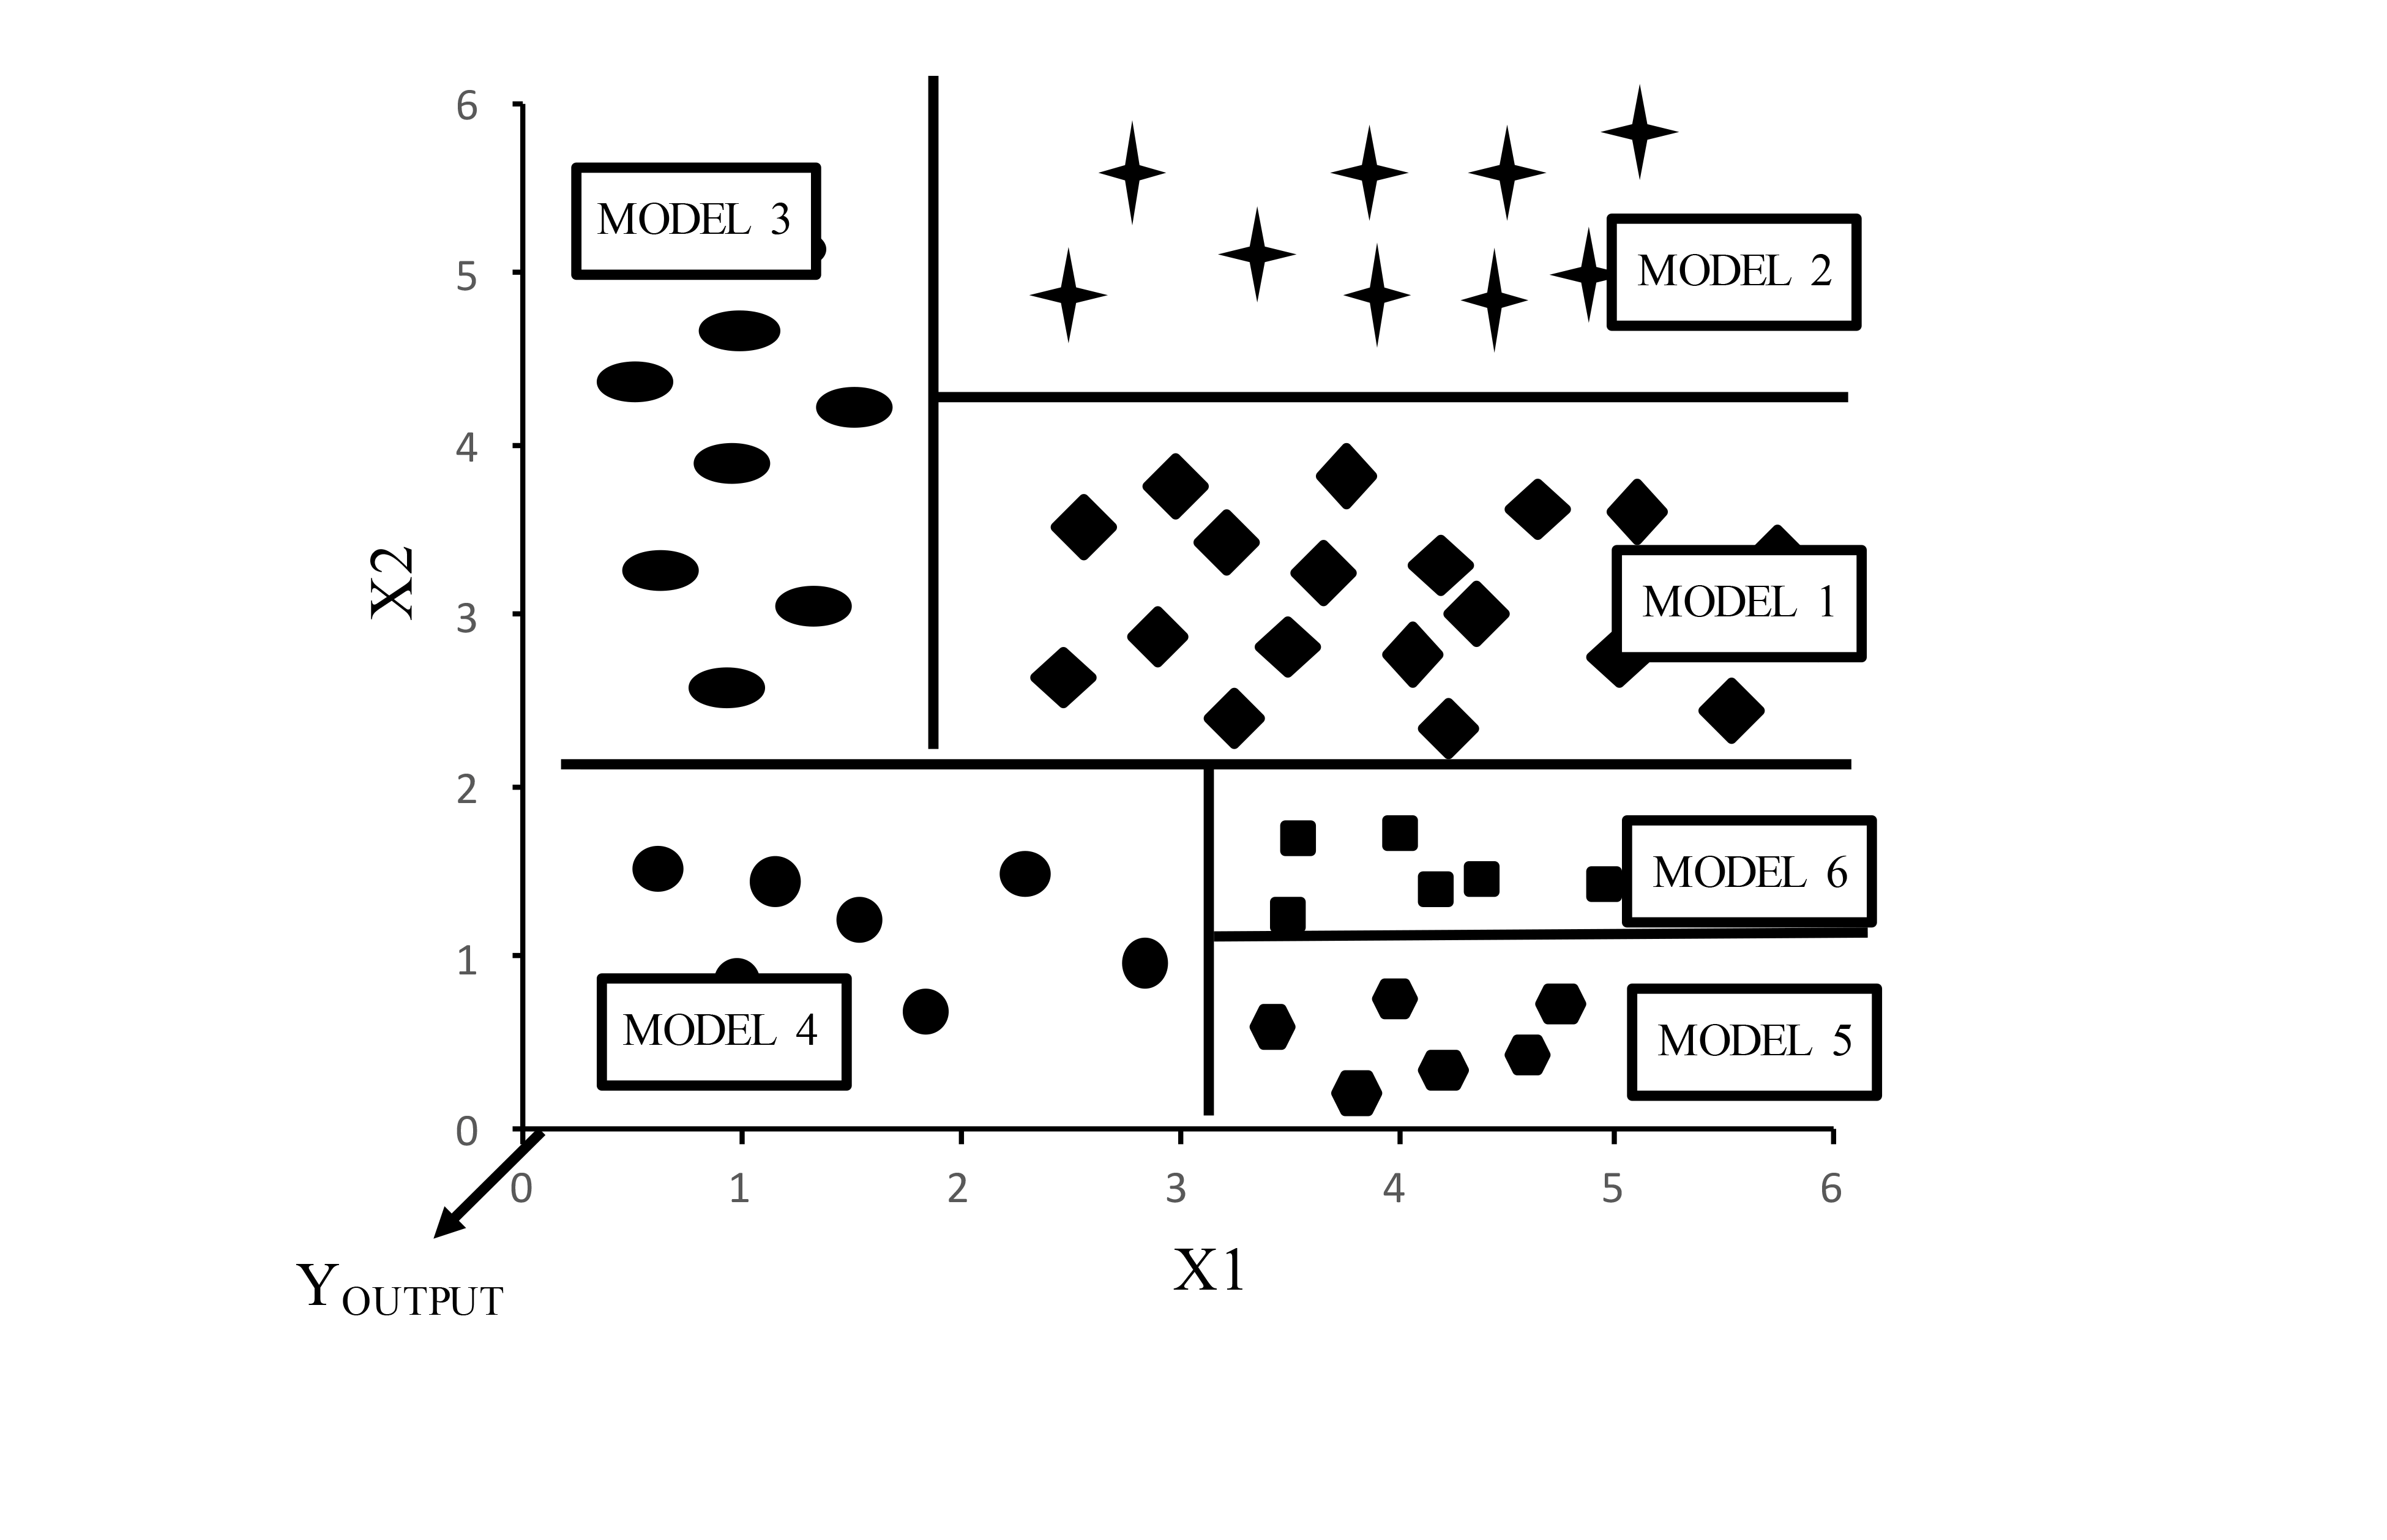
\includegraphics[height=7cm]{splits.png}
% \caption{Splitting of the input space (X1 x X2) by M5' model tree algorithm}
% \label{fig5}
% \end{figure}

% \section{Adding another section}
% You can show a lot of figures together like these Figures \ref{fig61}, \ref{fig62}, \ref{fig63} below.
% \begin{figure} [!htbp]
% \centering    
% \subfigure[Caption1]{\label{fig61}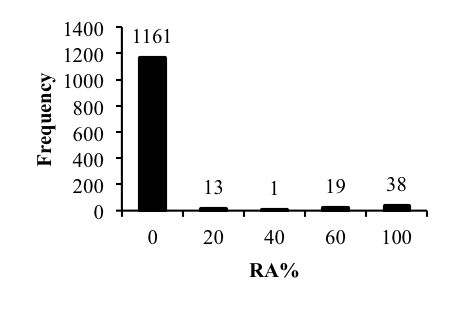
\includegraphics[width=42mm]{data1.png}}
% \subfigure[Caption2]{\label{fig62}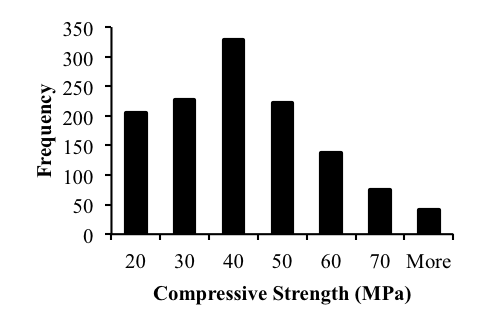
\includegraphics[width=42mm]{data2.png}}
% \subfigure[Caption3]{\label{fig63}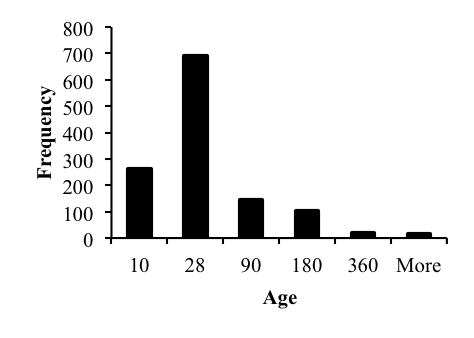
\includegraphics[width=42mm]{data3.png}}
% \caption{Figures sample}
% \end{figure}
% You can add lists into the text like this. 
% \begin{itemize}
% \settowidth{\leftmargin}{{\Large$\square$}}\advance\leftmargin\labelsep
% \itemsep3pt\relax
% \renewcommand\labelitemi{{\lower1pt\hbox{\small$\square$}}}
% \item	Some sample text item 1. 
% \item You may refer to tables \ref{tab1} 
% \item Or figures \ref{fig61}
% \end{itemize}

% Tables can be added like this
% \begin{table}[!htbp]
% \centering
% \caption{Sample table}
% \label{tab1}
% \begin{tabular}{llll}

% \hline
% Column 1 & Column 2 & Column 3       \\\hline
% 1         & Data1 & 13.41179 & 0.9492839 \\
% 2            & Data2 & 13.39824 & 0.9492952\\\hline
% \end{tabular}
% \end{table}




\addtocontents{toc}{\vspace{2em}} % Add a gap in the Contents, for aesthetics

% Solution Architecture - Discuss the solution architecture with reasoning at every step. AG will be there, so be very careful about using the distributed system terms and the solution that you are thinking of. 
% Chapter Template

\chapter{Solution Architecture} % Main chapter title

\label{Chapter 3} % Change X to a consecutive number; for referencing this chapter elsewhere, use \ref{ChapterX}

\lhead{Chapter 3. \emph{Solution Architecture}} % Change X to a consecutive number; this is for the header on each page - perhaps a shortened title

%----------------------------------------------------------------------------------------
%	SECTION 1
%---------------------------------------------------------------------------------------
\section{Assets in the network}

Our blockchain has two native asset types; a liquid asset type and an illiquid asset type. Let’s call the illiquid one BondCoin and the liquid one CashCoin. The blockchain has relatively small number of total coins; lets label this number maxCoins. Each coin is represented by a public-private key pair.

\subsection{BondCoins}

\begin{enumerate}
    \item To start with, a PoW consensus algorithm only mints BondCoins.
    \item After all the BondCoins have been minted, the PoW algorithm subsides and PoS takes over. Owners of BondCoins are the validators.
    \item The private-key of a BondCoin can be used to cast votes during the various phases of the BFT PoS consensus protocol. We can assume the BLS signature aggregation scheme as proposed in the ByzCoin paper for aggregating signatures of BondCoins.
    \item Each BondCoin is of unit denomination and cannot be divided into smaller values.
    \item There is a maturity duration d associated with each BondCoin, say a month. After d time, a BondCoin gets automatically converted into a CashCoin. As an important side benefit, the maturity duration helps in disabling voting rights of dormant BondCoins.
    \item The owner of each BondCoin can also convert it to a CashCoin before maturity but there is a penalty p associated with such a transaction. The convertor derives a value of [CashCoin - p] and p is distributed as fees to other validators.
    \item BondCoins accrue transaction fees for participating in the consensus process. The fees collected during each block are equally distributed among the BondCoins.
    \item BondCoins collectively determine, via consensus, the amount of fees to be charged for processing transactions. This is a key point. We will soon see that for any given number of BondCoins in the system, there is an equilibrium value for the fee amount to which it settles. Transaction validators can also force the fee value to a certain level in order to increase or decrease the number of validators in the system.

\end{enumerate}

\subsection{Benefits of holding BondCoins}

\begin{enumerate}
    \item Storage: Risk free time shifting of value.
    \item Earn Fees: Holders of BondCoin earn a fraction of the transaction fees.
    \item Speculation: BondCoin prices will fluctuate constantly. Speculators that believe that the BondCoin prices are low can buy them.
\end{enumerate}

\subsection{Costs of holding BondCoins}

Holding BondCoins will lead to loss of liquidity. And, to convert them back before maturity would lead to penalty. So, BondCoins act as fixed deposit, you gain interest on them over their maturity period. But you can only take them out once they are fully matured. Otherwise, you will have to compromise with the interest(penalty).

\subsection{CashCoins}

\begin{enumerate}
    \item CashCoins can exist in any denominations and hence are very liquid. You can buy coffee with CashCoin.
    \item Fractions of CashCoin can be accumulated into a unit of CashCoin and further converted into a unit of BondCoin by the owner.
\end{enumerate}

\subsection{Benefits of holding CashCoins}

CashCoins are highly liquid. They can be used in following manner :

\begin{enumerate}
    \item Transactions: People will hold CashCoins to buy goods and services.
    \item Precautions: People will hold CashCoins for contingencies like medical emergencies or the sudden loss in value of a national currency.
    \item Speculation: Speculators that believe that the BondCoin prices are too high can sell them and hold CashCoins instead guarding against possible drops in value of BondCoin.
\end{enumerate}

\subsection{Costs of holding CashCoins}

The price of holding CashCoins is the transaction fees. As these coins could have levied transaction fees while they were not being used. Similar to interests that we gain while keeping our money in a bank.

\section{Market Dynamics}
What we have created with the dual asset types concept is a wonderful interplay between the demand for CashCoins, the demand for BondCoins and the transaction fees. Lets understand the interplay between CashCoins, BondCoins and transaction fees better by noting the costs and benefits of holding either. This is very similar to the interplay between the demand for cash, the demand for bonds and the central bank determined interest rate.

\subsection{Demand Curve for CashCoin}

\begin{figure} [!htbp]
\centering    
\subfigure[Demand Curve for CashCoin]{\label{fig31}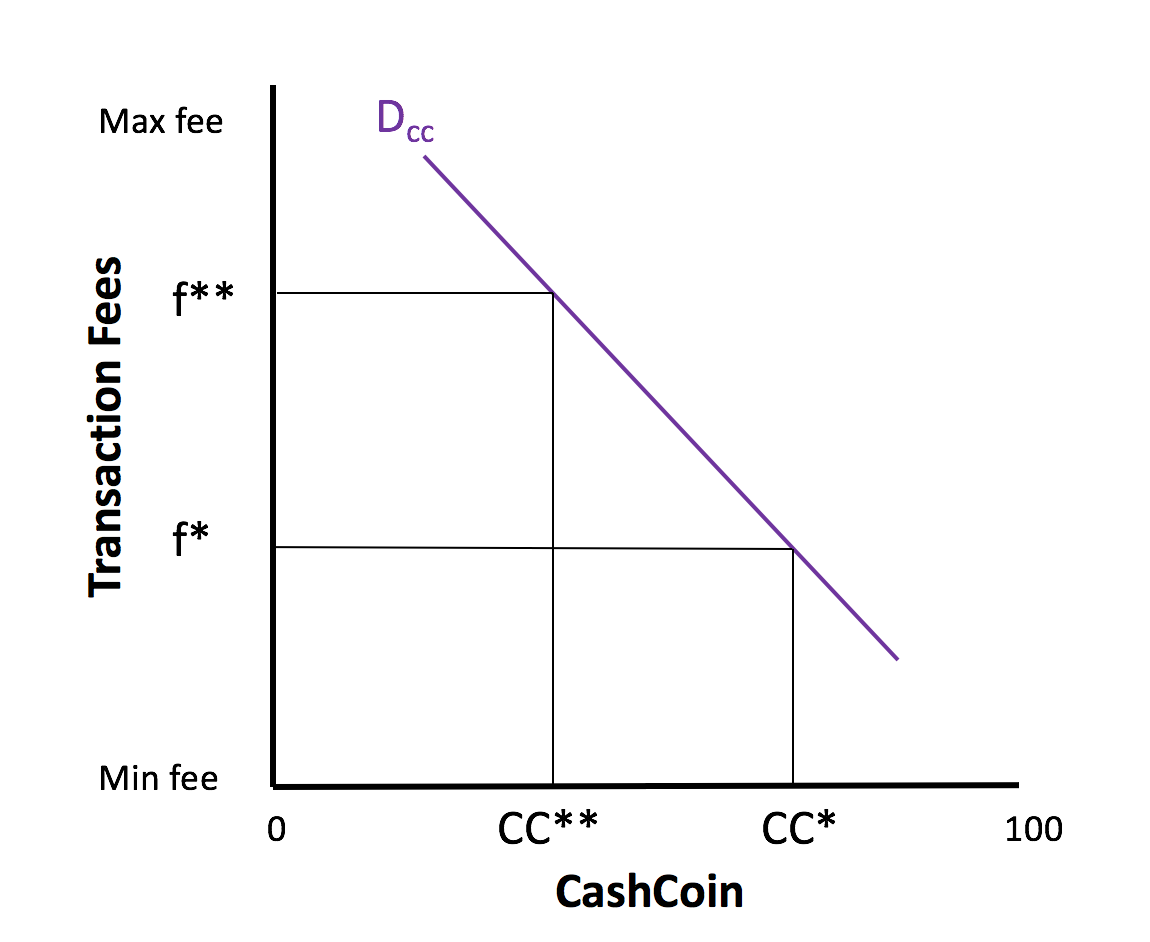
\includegraphics[width=7cm]{dcfc.png}}
\subfigure[Change in demand for CashCoin]{\label{fig32}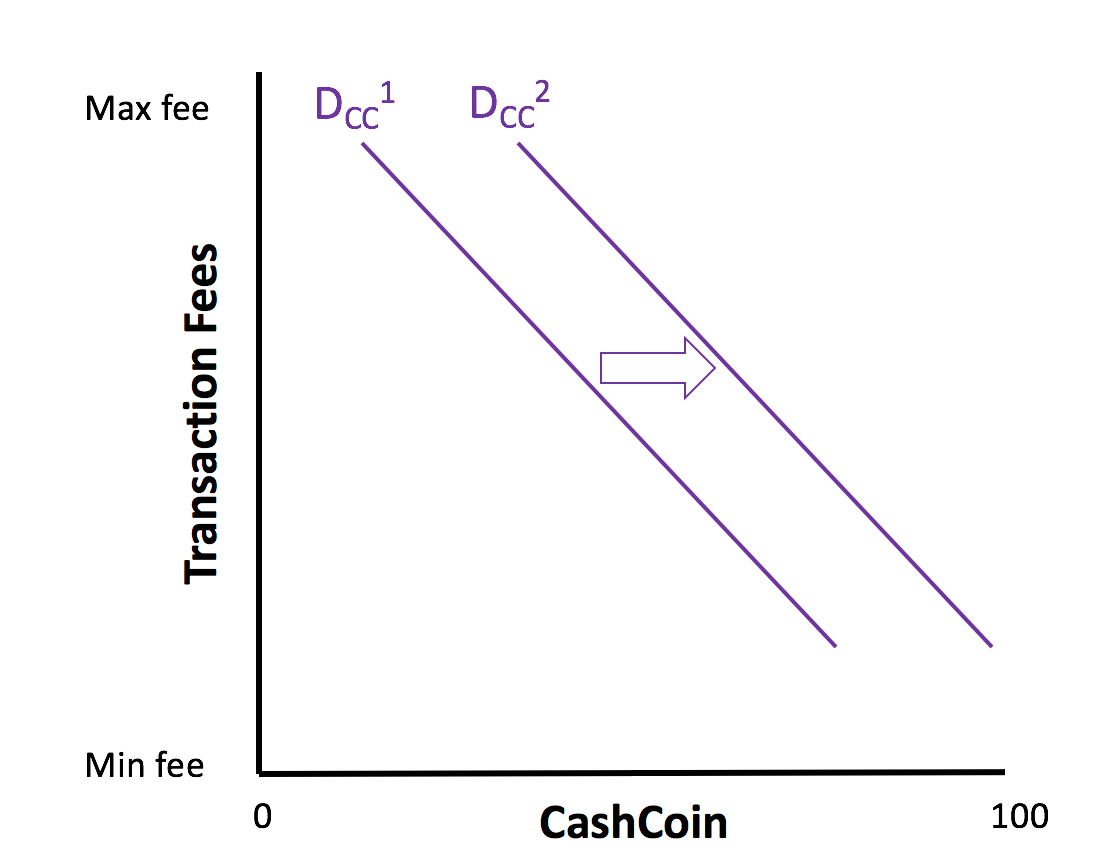
\includegraphics[width=7cm]{cidfc.png}}
\caption{Dynamics of CashCoin}
\end{figure}

The various sources of demand for CashCoins (transactions, precautionary and speculative) will vary negatively with transaction fees. An additional source of demand for CashCoins is from participants wanting lesser decentralization, faster throughputs and lower fees. Let’s label this demand as the higher network performance demand. Lower the fees, higher the demand for CashCoins.

Lets suppose CC** is the total amount of CashCoins at some point in time. I.e., CC** is the supply of CashCoins. Then, the CashCoin market equilibrium will occur at transaction fee f** where the demand meets supply. Now, suppose CashCoin availability increases to CC*, the market equilibrium will occur at transaction fee f* where the demand curve meets the new supply.

\subsection{Change in Demand for CashCoin}

Previously, we have identified 4 sources of demands for CashCoins. i) transactions demand, ii) precautionary demand, iii) speculative demand and iv) higher network performance demand. The various sources of demand for CashCoins can change. For example, during festivals in light of higher retail spending, the transaction demand may rise moving the demand curve as shown in the above figure.

\subsection{Demand Curve for BondCoin}

The various sources of demand for BondCoins (storage, fees and speculative) will vary positively with transaction fees. An additional source of demand for BondCoins is from participants wanting more decentralization and who do not mind paying higher fees. Let’s label this demand as the higher decentralization demand. Higher the fees, higher the demand for BondCoins.

\begin{figure} [!htbp]
\centering    
\subfigure[Demand Curve for BondCoin]{\label{fig33}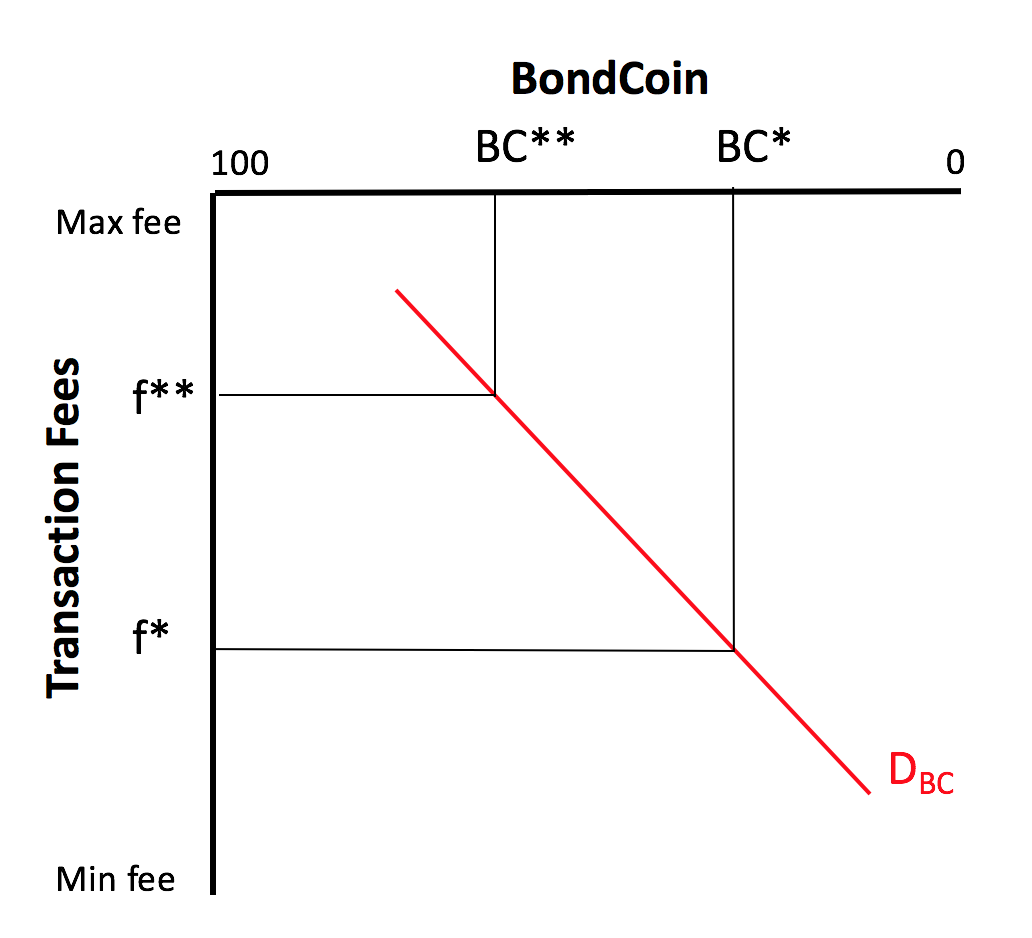
\includegraphics[width=7cm]{dcfb.png}}
\subfigure[Change in demand for BondCoin]{\label{fig34}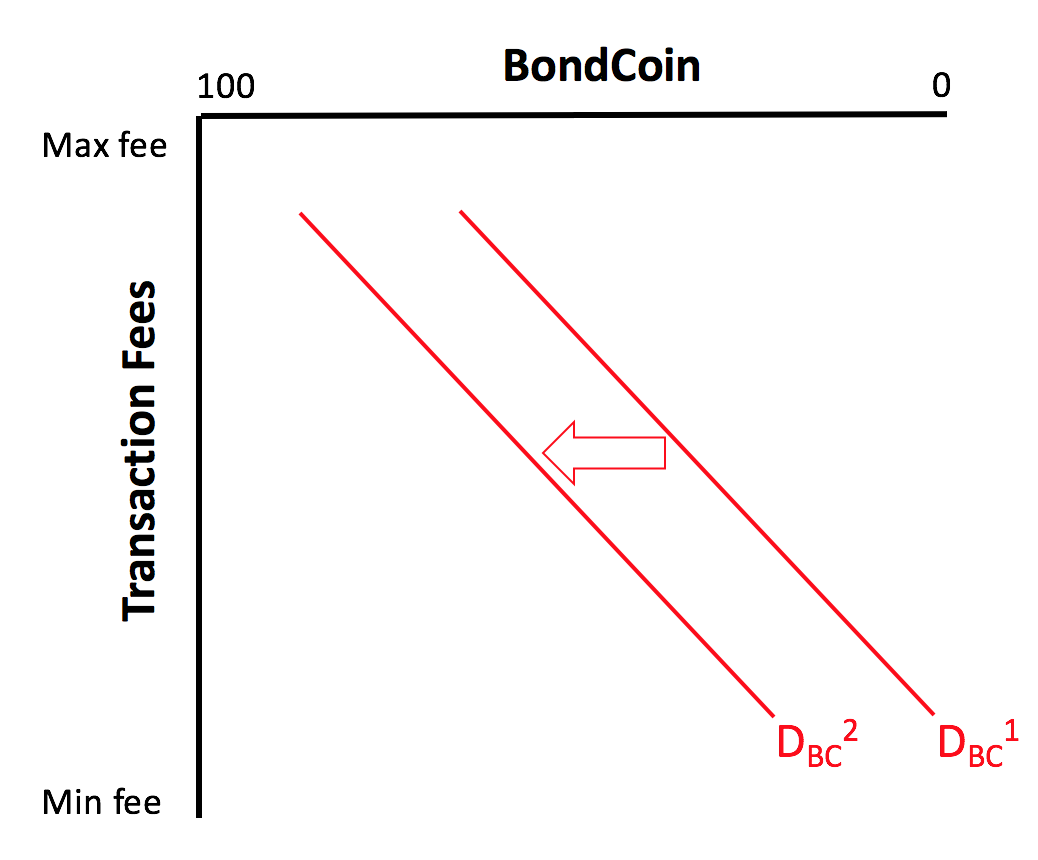
\includegraphics[width=7cm]{cidfb.png}}
\caption{Dynamics of BondCoin}
\end{figure}

Lets suppose BC* is the total number of BondCoins at some point in time. I.e., BC* is the supply of BondCoins. Then, the BondCoin market equilibrium will occur at transaction fee f* where the demand meets supply. Now, suppose BondCoin availability increases to BC**, the market equilibrium will occur at transaction fee f** where the demand curve meets the new supply.

\subsection{Change in Demand for BondCoin}

Previously, we have identified 4 sources of demands for BondCoins. i) storage demand, ii) fees demand, iii) speculative demand and iv) higher decentralization demand. The various sources of demand for BondCoins can change. For example, if the transaction fees increase in anticipation of subdued transaction volumes, the fee demand may rise moving the demand curve as shown in the above figure.

\section{The Common Market Equilibrium}

The supply of BondCoins is simply maxCoins - supply of CashCoins. As shown below, it can be represented by a single line. The supply curve intersects with the demand curves of CashCoin and BondCoin at the same point. This is the common market equilibrium for both CashCoins and BondCoins. There is of course a single fee value f for this common market equilibrium.

\begin{figure}[!htbp]
\centering
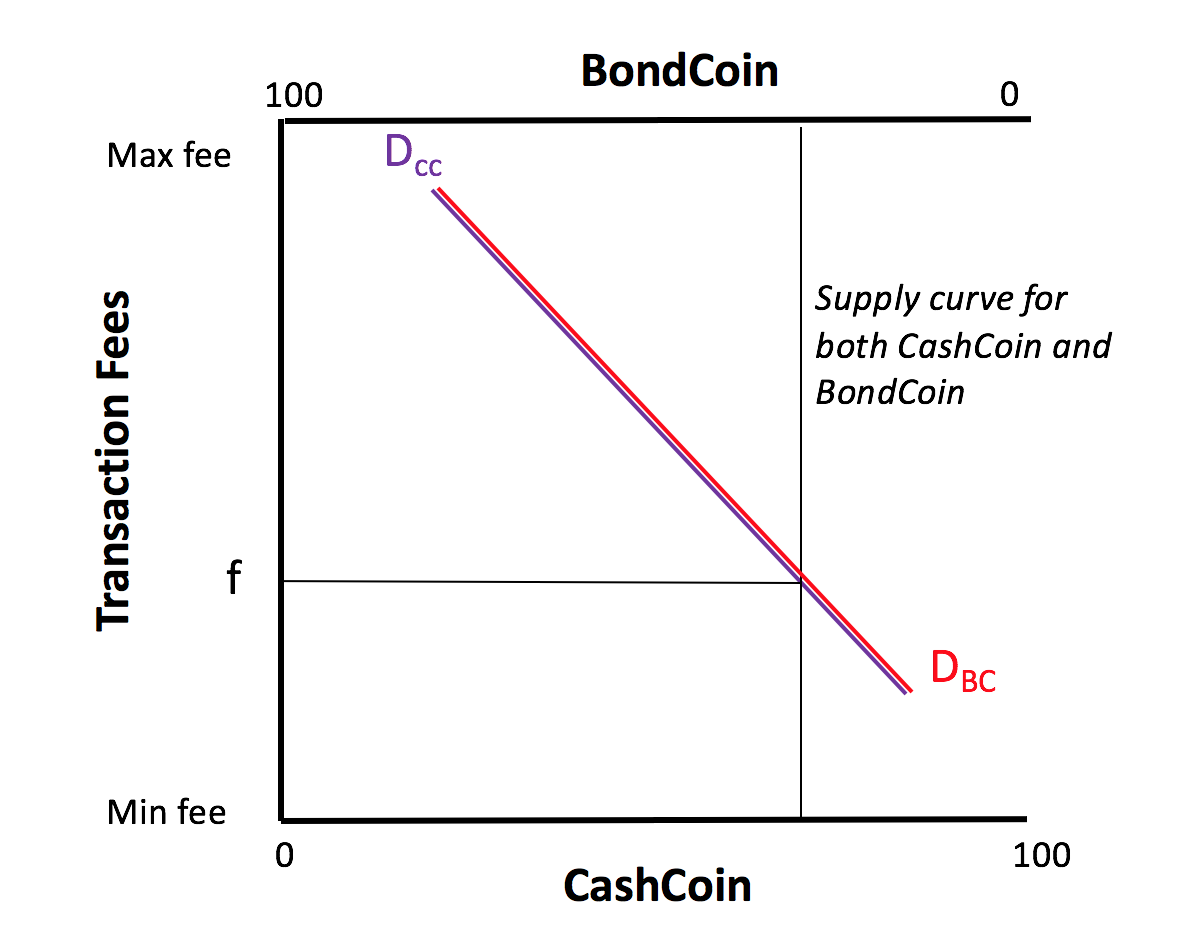
\includegraphics[height=10cm]{tcme.png}
\caption{The Common Market Equilibrium}
\label{fig35}
\end{figure}

This common market equilibrium represents the steady state of the system that respects the aggregate demands and supplies for CashCoin and BondCoin. The number of BondCoins at this equilibrium represent the number of validators in the blockchain.

\addtocontents{toc}{\vspace{2em}} % Add a gap in the Contents, for aesthetics

% Discussion - Discuss the issues that you have got in the system, an idea about how you are trying to solve those. 
% Chapter Template

\chapter{Discussion} % Main chapter title

\label{Chapter 4} % Change X to a consecutive number; for referencing this chapter elsewhere, use \ref{ChapterX}

\lhead{Chapter 4. \emph{Discussion}} % Change X to a consecutive number; this is for the header on each page - perhaps a shortened title

\section{Problems in System Design}

Here, we note some of the problems and boundary cases that might occur during the design and execution of the system and we try to give some plausible solutions.

\begin{enumerate}
    \item We know that CashCoins are liquid and can be transferred from one user to another. But, what if a user wants to transfer his voting rights to another user? If this user simply transfers it then he would also have to share the public-private key associated with this coin, but these are digital quantities and can be copied and can lead to the free-rider problem.\\
    Solution : Here, we assume that BondCoins are illiquid and non-transferable. If some user wants to transfer them, then he first has to convert the Coin to CashCoin and send these to the target user who then can convert these back to a BondCoin. This also avoids the free rider problem as when the target user gets his BondCoin, he would also get a new key pair associated with it.
    \item The bond coins are going to be minted using PoW. Once, all the bond coins are minted, the system adopts PoS system. PoW means we are finding some nonce which satisfies some properties, (In case of bitcoin, it had to be less than a given number). But, here the each bond coin is associated with a public and a private key pair which satisfy their own properties. How does the two gets associated?\\
    Solution : Here, the nonce and key-pairs are not related. A user can get a key pair even when PoS has taken over. We use El Gamal Cryptosystem for getting the private-public key pair associated with the BondCoin. This Cryptosystem is based on Elliptic Curve Cryptography (ECDLP) and provides better security with lesser key size. The Base point is common for all users. The private key can be decided by the winner of the current round randomly and based on it a public key can be chosen. But, once its decided, the user cannot change it and has to wait till the BondCoin matures. If he wants to change it then he would have to convert it to CashCoin and then again to BondCoin to choose a new one.
    \item What happens if a user who already owns a BondCoin wins another round while PoW consensus is active?\\
    Solution : If a user wins another round while PoW consensus is active, then he gets to commit that block but the BondCoin that is minted gets added to his account as CashCoin without any penalty. This is done to make sure that each validators has equal voting rights and hence own only one BondCoin with them.
    \item Here we note that PoW algorithm is only for minting bond coins. So, do the users don’t transact till all the bond coins are minted or does the peer minting the next bond coin becomes the leader for that round and commits the block of transactions to the ledger and once all the minting is over, PoS takes over and only those peers can take part in validation who are holding the bond coins?\\
    Solution : Here, we go with the choice that when the PoW consensus is active, the users can still transact and transaction fees are not taken from them. This is done to invite new users to the system and to increase the validators in the system. To incentivise users to participate in the consensus, the BondCoin minted in the current round is paid to the winner of the current round. Note that even after winning once, the users would still want to participate in the consensus to increase the CashCoins in their account.
    \item Each BondCoin comes with a maturity duration d. How is this maturity duration decided? What happens to the keys of the BondCoin once it gets expired and gets converted into CashCoin?\\
    Solution : Currently, this maturity duration is kept as a constant. Eg: 1 month. And, we plan to decide this value emphirically. Each BondCoin comes with a manufacture date, which is stored in the ledger. Once a BondCoin is expired, it gets added as CashCoins to the user account and the keys become useless. This process takes place the first time user transacts after his BondCoin is expired. If he tries to vote using the old keys then his vote is discarded during the expiration check phase.
    \item Since, the CashCoins are not converted automatically to BondCoins, what happens when there is no BondCoin left in the system?\\
    The situation where no BondCoins are left in the system is hard to occur. As the BondCoins in the system decrease, the transaction fees would decrease. In this case, automatically the demand for BondCoins would increase as the few users who are owners of the last few BondCoin would enjoy more shares of the transaction fees by themselves. But, no BondCoin situation can occur only when the last of BondCoins also got matured automatically and no other user converted their CashCoin into a BondCoin before their expiration which would bring the system to a standstill. If there are no BondCoin in the system then there would be no validators in the system and no user would be able to transact and hence the CashCoins in their account would become useless. In this unlikely situation, we suggest that the PoW system is restarted so that the BondCoins in the system can be increased and users can enjoy transactions without paying the fees and do not have to leave the system.
    \item Why is there a penalty for converting BondCoin to CashCoin? How is its amount fixed?\\
    Solution : The BondCoin is like a contract given to user to participate in the validation process during its maturity period. Its like a fixed deposit done in bank, on which you get the interest during the period but you can use the money only after it matures, if you take the money out before it matures then you have to pay a penalty. In a similar way, this penalty is imposed on those users who want to do away with their responsibility of participating in the validation process. The amount is fixed based on the number of BondCoins currently in the system. More the number of BondCoins, more the penalty.

\end{enumerate}

\section{Plausible attacks}

Here, we assume that the block has been prepared and validators are decided, we only need to consider attacks that can be made while committing this block to the ledger.

\begin{enumerate}
    \item Adversary can be the owner of majority of bond coins. Adversary can make multiple accounts with only enough cash coin to convert them into bond coins.
    \item If in response to above, the bond coins are made larger in number then network attacks would be easier. Adversary may be able to slow down the network or partition some nodes.
    \item Instead of buying the bond coins itself, adversary may hack prominent accounts holding bond coins. It's useful as they are gonna be valid for duration d.
\end{enumerate}

\addtocontents{toc}{\vspace{2em}} % Add a gap in the Contents, for aesthetics

% Conçlusion and Future Works. 
% Chapter Template

\chapter{Conclusion and Future Works} % Main chapter title

\label{Chapter 5} % Change X to a consecutive number; for referencing this chapter elsewhere, use \ref{ChapterX}

\lhead{Chapter 5. \emph{Conclusion and Future Works}} % Change X to a consecutive number; this is for the header on each page - perhaps a shortened title

In this report, we saw how the number of validators for a POS system can be dynamic and may be determined by the market parameters. The POS systems were better than POW systems because they don't waste computational power in redundant tasks but POS systems itself has some drawbacks. The proposed system tries to solve some of these drawbacks. The crux of the proposed system lies in the fact that all the validators are given equal voting rights so that adversary is also ripped off of the probabilistic advantage of gaining the control of the system which is prevalent in the recently proposed systems such as Algorand. In this system, gaining half the currency of the system is not enough for the adversary. He must have control over more than half of the BondCoins i.e. more than half of the computation power. And, as these BondCoins come with an expiry, the task of the adversary becomes more difficult.

In future we would like to achieve the following objectives :
\begin{enumerate}
    \item We would like to explore how the system is affected if the maturity duration of a BondCoin is variable
    \item We would like to devise a method to ensure that a minimum number of validators are always there in the network at a given point of time
    \item We would like to explore how the system is affected if the BondCoin is also quantized. For eg : a group of users can combine their CashCoins to get one BondCoin. What would be the final vote of such a group of users?
    \item Till now, we have assumed that all the validators remain active all the time. We would like to explore what happens if some of the validators crash or go offline.
    \item We would like to tackle the geographical scalability of POS protocols and devise a solution for it.
    \item We would like to implement a prototype of the above proposed system and run benchmark tests on it.
    \item We would like to explore how charging fees for conversion of CashCoin to BondCoin affects the economy of the system.
\end{enumerate}


\addtocontents{toc}{\vspace{2em}} % Add a gap in the Contents, for aesthetics

% \appendix % Cue to tell LaTeX that the following 'chapters' are Appendices

% % Include the appendices of the thesis as separate files from the Appendices folder
% % Uncomment the lines as you write the Appendices

% % Appendix Template

\chapter{Appendix A} % Main appendix title

\label{AppendixX} % Change X to a consecutive letter; for referencing this appendix elsewhere, use \ref{AppendixX}

\lhead{Appendix X. \emph{Appendix Title Here}} % Change X to a consecutive letter; this is for the header on each page - perhaps a shortened title

Write your Appendix content here.

% %\input{Appendices/AppendixB}
% %\input{Appendices/AppendixC}

% \addtocontents{toc}{} % Add a gap in the Contents, for aesthetics

%\backmatter

%----------------------------------------------------------------------------------------
%	BIBLIOGRAPHY
%----------------------------------------------------------------------------------------
%\nocite{*}
\clearpage

%\addtotoc{Acknowledgements}
%\thispagestyle{plain}


\chapter{References} % Main chapter title

\label{References} % Change X to a consecutive number; for referencing this chapter elsewhere, use \ref{ChapterX}

\lhead{\emph{References}} % Change X to a consecutive number; this is for the header on each page - perhaps a shortened title


%\label{References}

%\btypeout{References}
%\begin{center}{\huge{\textit{Acknowledgements}} \par}\end{center}

%\lhead{\emph{References}} % Change the page header to say "Bibliography"


%\addtotoc{References}

%\bibliographystyle{apalike} % Use the "custom" BibTeX style for formatting the Bibliography

%\bibliography{Bibliography} % The references (bibliography) information are stored in the file named "Bibliography.bib"

\begin{enumerate}
    \item S. Nakamoto, Bitcoin: A Peer-to-Peer Electronic Cash System, 2008.
    \item S. Liu, P. Viotti, C. Cachin, V. Quéma, M. Vukolic, "XFT: practical fault tolerance beyond crashes", Proc. 12th USENIX OSDI, 2016.
    \item Y. Gilad, R. Hemo, S. Micali, G. Vlachos, N. Zeldovich, "Algorand: Scaling Byzantine Agreements for Cryptocurrencies", Cryptology ePrint Archive Report 2017/454, 2017.
    \item https://en.wikipedia.org/wiki/State\_machine\_replication
    \item https://en.wikipedia.org/wiki/Blockchain
    \item https://medium.com/@deshpande.pralhad/a-proof-of-stake-blockchain-with-two-native-asset-types-35f643bb3ff3
    \item https://open.lib.umn.edu/principleseconomics/chapter/25-2-demand-supply-and-equilibrium-in-the-money-market/
    \item https://medium.com/coinmonks/understanding-proof-of-stake-the-nothing-at-stake-theory-1f0d71bc027
    \item https://lisk.io/academy/blockchain-basics/how-does-blockchain-work/proof-of-stake
\end{enumerate}

\end{document}  
